\documentclass[handout]{beamer}
\usepackage{bm}
\usepackage{colortbl}
\usepackage{listings}
\usepackage{algorithmic}
\usepackage{verbatim}
\usepackage{rotating}
\usepackage{booktabs}
\usepackage{multirow}
\lstloadlanguages{R}
\lstset{ language=R, basicstyle=\scriptsize\ttfamily, commentstyle=\ttfamily\color{gray}, numbers=left, numberstyle=\ttfamily\color{gray}\footnotesize, stepnumber=1, numbersep=5pt, backgroundcolor=\color{white}, showspaces=false, showstringspaces=false, showtabs=false, frame=single, tabsize=2, captionpos=b, breaklines=true, breakatwhitespace=false, escapeinside={}, keywordstyle={}, morekeywords={} }\renewcommand{\P}{\mathcal{P}}
\newcommand{\bt}{\pmb{\theta}}
\newcommand{\bG}{\pmb{\Gamma}}
\newcommand{\p}{\pause}
\newcommand{\pitem}{\pause \item}
\newcommand{\N}{\mathcal{N}}
\newcommand{\Y}{\bm{\mathcal{Y}}}
\newcommand{\bh}{\bm{h}} 
\DeclareMathOperator*{\argmax}{arg\,max}

\usefonttheme{serif}

\newenvironment{changemargin}[2]{%
  \begin{list}{}{%
    \setlength{\topsep}{0pt}%
    \setlength{\leftmargin}{#1}%
    \setlength{\rightmargin}{#2}%
    \setlength{\listparindent}{\parindent}%
    \setlength{\itemindent}{\parindent}%
    \setlength{\parsep}{\parskip}%
  }%
  \item[]}{\end{list}} 

%
\title{Inferential Analysis of the  \\ Supreme Court Citation Network}
%
\definecolor{umassred}{HTML}{001769}
\setbeamercolor{structure}{fg=umassred} 
\author{ \textbf{Bruce A. Desmarais}\\ Collaborators: Christian Schmid, Ted Chen, David Hunter \\~\\ {\bf Pennsylvania State University}}



\begin{document}
%\date{November 16, 2012}

\begin{frame}
\vspace{1cm}
  \titlepage
  \vspace{0cm}
  \begin{center}
   \begin{tabular}{cc}
\hspace*{-.2in} \tiny \begin{minipage}{3.5in}
Work supported by NSF grants SES-1558661, SES-1619644, SES-1637089, and CISE-1320219)\\ ~\\~\\~\\~\\
\end{minipage}
& \includegraphics[scale=.05]{figures/NSF_logo.png}
\end{tabular}
\end{center}
\end{frame}

\begin{frame}[plain]% \frametitle{The Importance of Precedent}
\centering

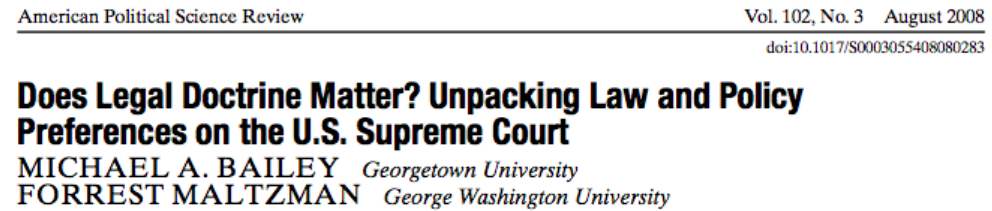
\includegraphics[width = 0.9\textwidth ]{../../images/apsrReference}
\\
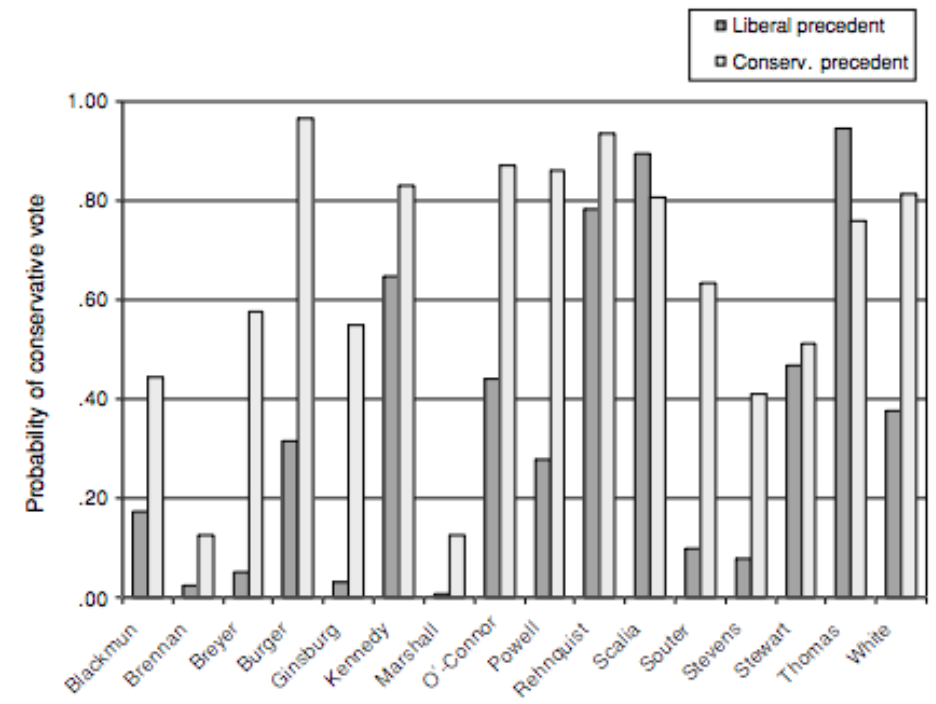
\includegraphics[width = 0.9\textwidth ]{../../images/apsrTableScreenshot}
\end{frame}

\begin{frame} \frametitle{Two Limitations in Case-Level Analysis}
\Large
\begin{enumerate}
\item {\bf Theoretical:} Cannot learn about relational processes
\\~\\
\item {\bf Methodological:} Risk bias from omitted structure
\end{enumerate}

\end{frame}

\begin{frame} \frametitle{Reciprocity}

\centering

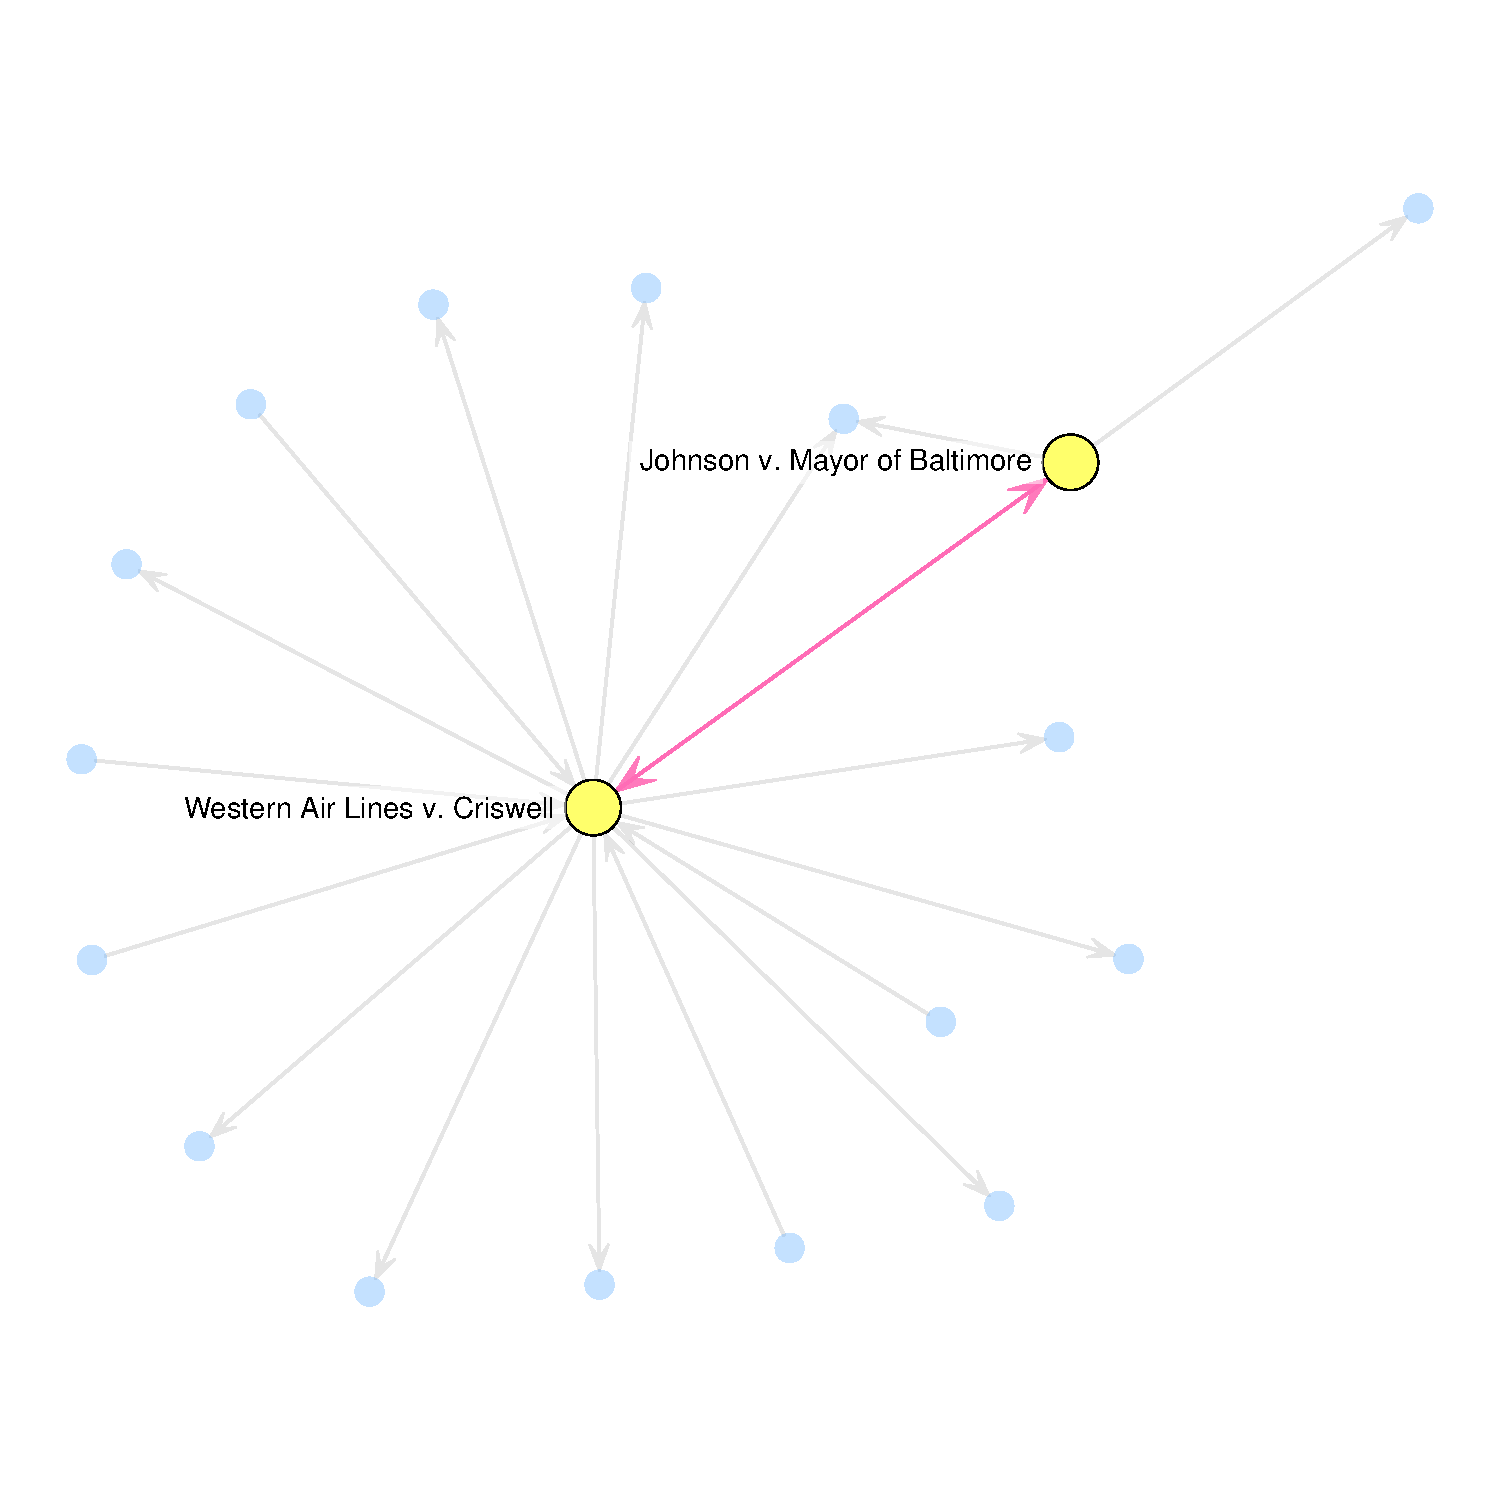
\includegraphics[width = 0.95\textwidth,trim= 0cm 1cm 0cm 2cm,clip=true ]{../../../NetworkVisualizations/citations_recip.pdf}

\end{frame}

\begin{frame} \frametitle{Transitivity}
\centering

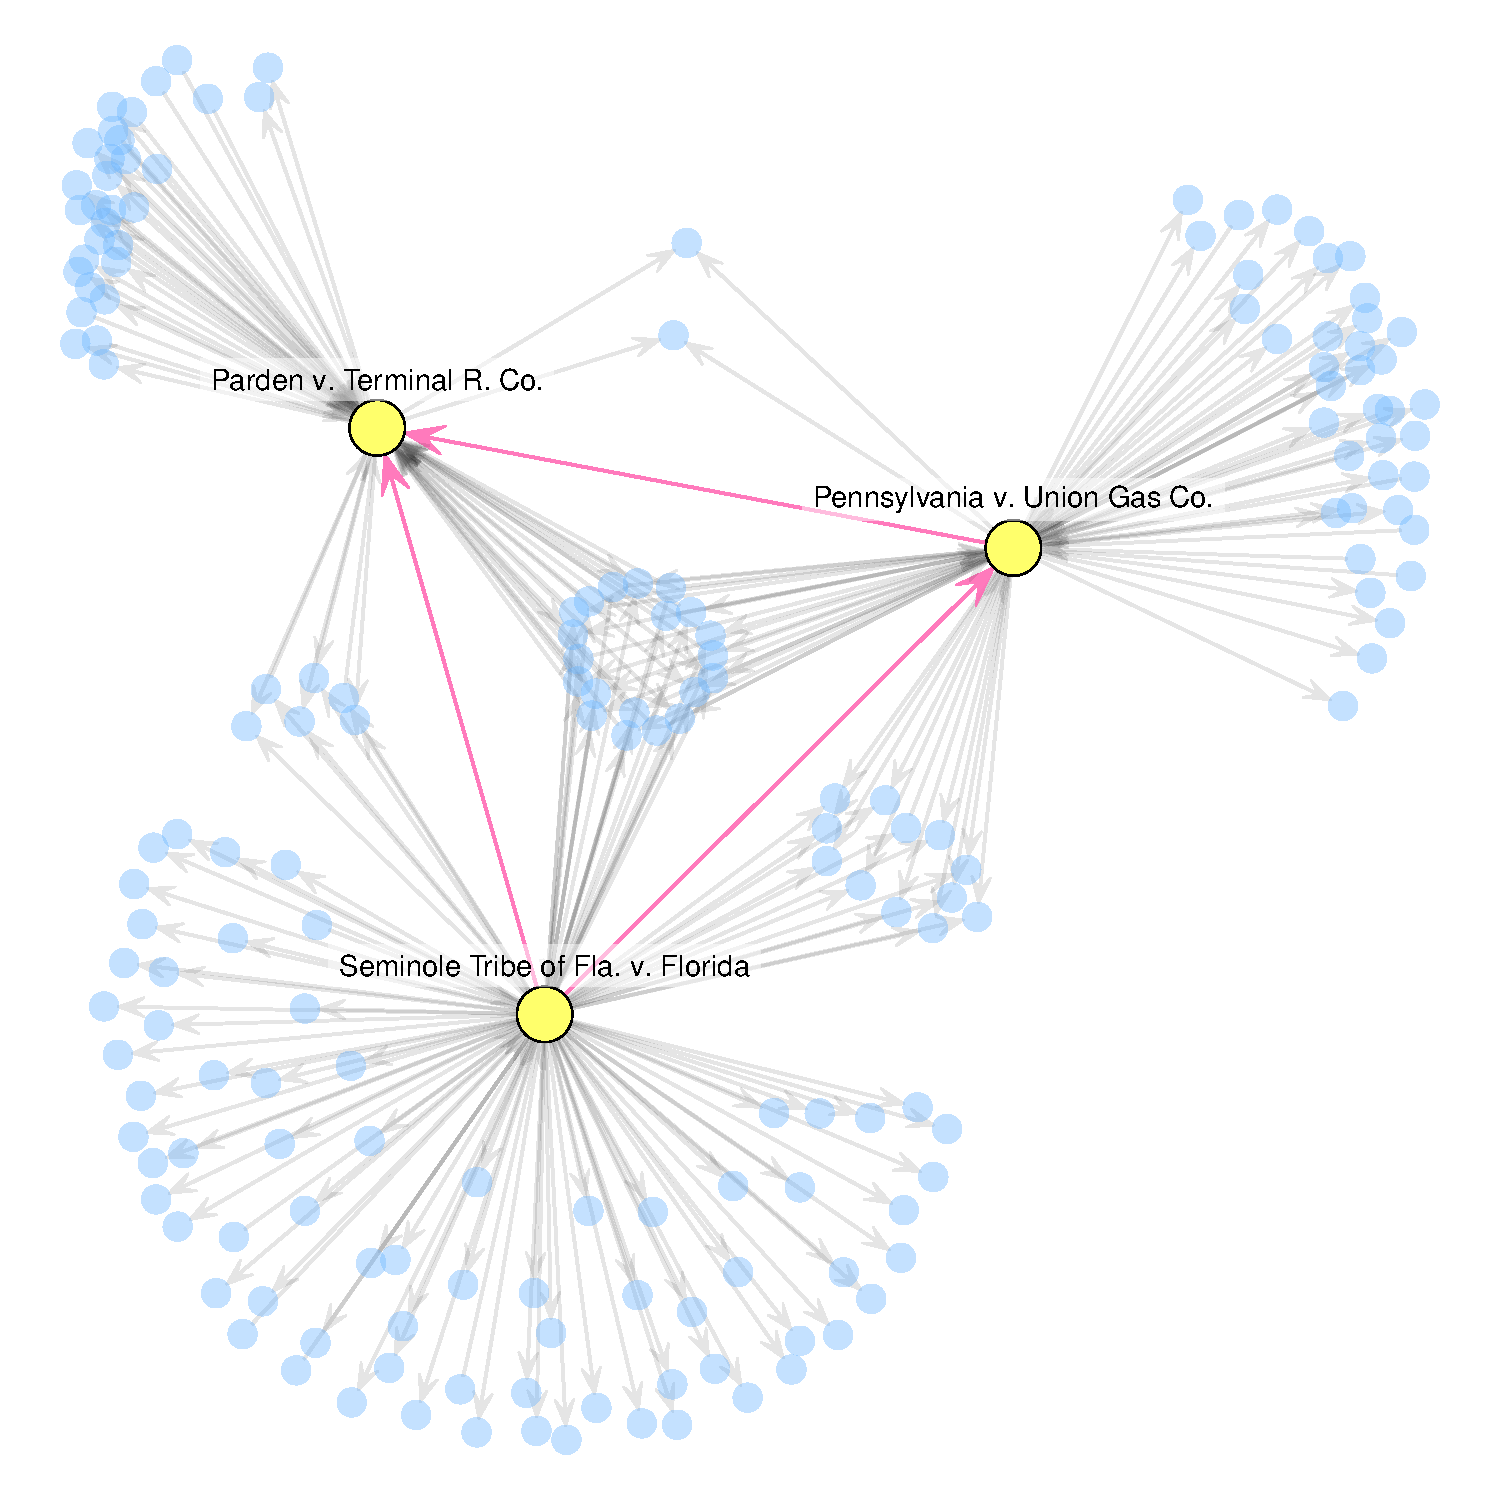
\includegraphics[width = 0.95\textwidth,trim= 0cm 1cm 0cm 2cm,clip=true ]{../../../NetworkVisualizations/citations_trans.pdf}

\end{frame}

\begin{frame} \frametitle{Popularity and Activity}

\centering

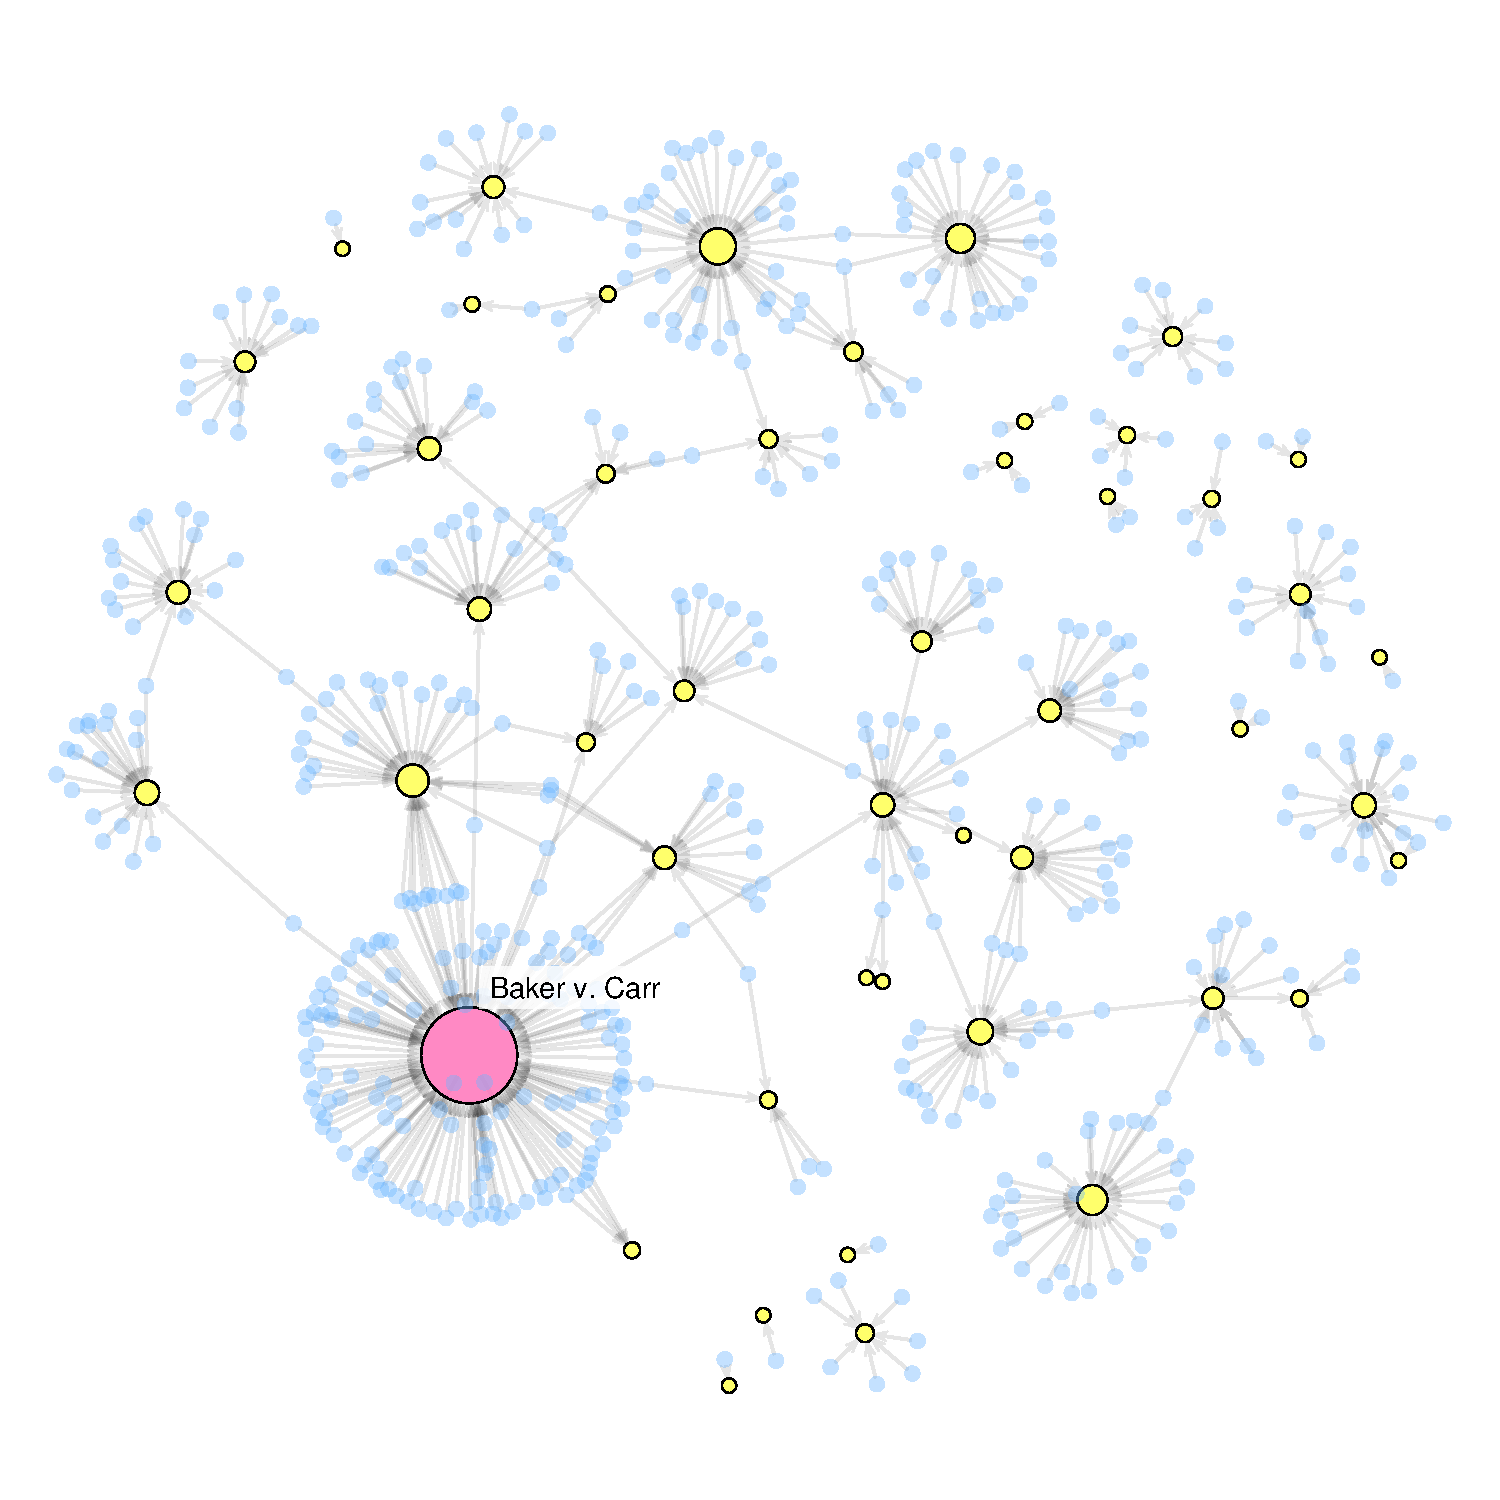
\includegraphics[width = 0.95\textwidth,trim= 0cm 3cm 6cm 8cm,clip=true ]{../../../NetworkVisualizations/citations_pop.pdf}


\end{frame}





\frame{
\frametitle{Citation Temporal Exponential Random Graph Model}\vspace{0.5cm}

The probability  of observing the $N_t \times N_{\leq t}$ adjacency matrix $C_t$ given past citations $C_{<t}$, where $C_{\leq t}$ is the network up to time $t$
\[
\mathcal{P}(C_t|C_{<t}, \bt) = \frac{\exp \{ \bt' \bh(C_{\leq t})  \}}{\sum_{C^*_t \in \mathcal{C}_t} \exp \{\bt ' \bh(C^*_{\leq t})\}  }
\]
Decomposition:
\[
\underbrace{\bh(C_{\leq t})}_{Net\hspace{3pt} Stats} \qquad \underbrace{\bt}_{Effects} \qquad \underbrace{\exp \{\bt' \bh(C_{\leq t}) \}}_{+ \hspace{3pt} Weight} \qquad \underbrace{\sum_{C^*_t \in \mathcal{C}_t} \exp \{\bt ' \bh(C^*_{\leq t})\}}_{Normalizer}
\]

Flexible: $\bh$ can capture virtually any form of interdependence among the edges $+$ covariates\\
\vspace{0.5cm}
Normalizing constant can make estimation difficult
}

\begin{frame} \frametitle{DAG[gish] Dynamics}
\centering

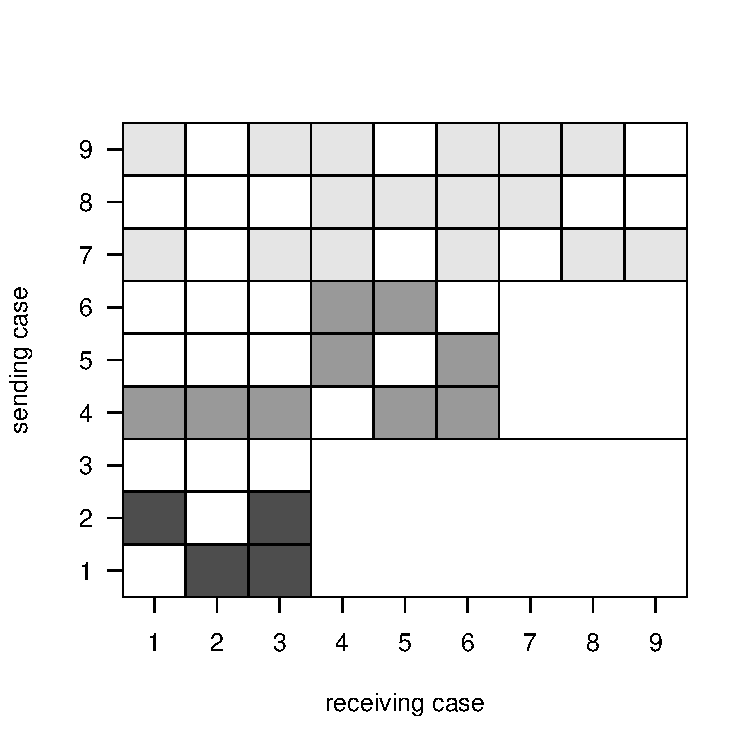
\includegraphics[width = 0.95\textwidth,trim= 0cm 0cm 0cm 0cm,clip=true  ]{../../../Tex/images/daggish.pdf}

\end{frame}




\begin{frame} \frametitle{Data}

\begin{columns}
\begin{column}{4cm}
\scalebox{0.8}{
\begin{tabular}{|
>{\columncolor[HTML]{C0C0C0}}l |l|l|}
\hline
{\color[HTML]{333333} } & \cellcolor[HTML]{C0C0C0}{\color[HTML]{333333} Terms} & \cellcolor[HTML]{C0C0C0}{\color[HTML]{333333} Cases} \\ \hline
CE Hughes*              & 1937 - 1941                                          & 629                                                                                                                  \\ \hline
HF Stone                & 1942 - 1946                                          & 766                                                                                                                \\ \hline
FM Vinson               & 1946 - 1953                                          & 788                                                                                                                  \\ \hline
E Warren                & 1954 - 1969                                          & 2159                                                                                                                  \\ \hline
WE Burger               & 1970 - 1986                                          & 2805                                                                                                                   \\ \hline
W Rehnquist**            & 1987 - 2001                                          & 1670                                                                                                                 \\ \hline
\end{tabular}
}
\end{column}
\begin{column}{6cm}
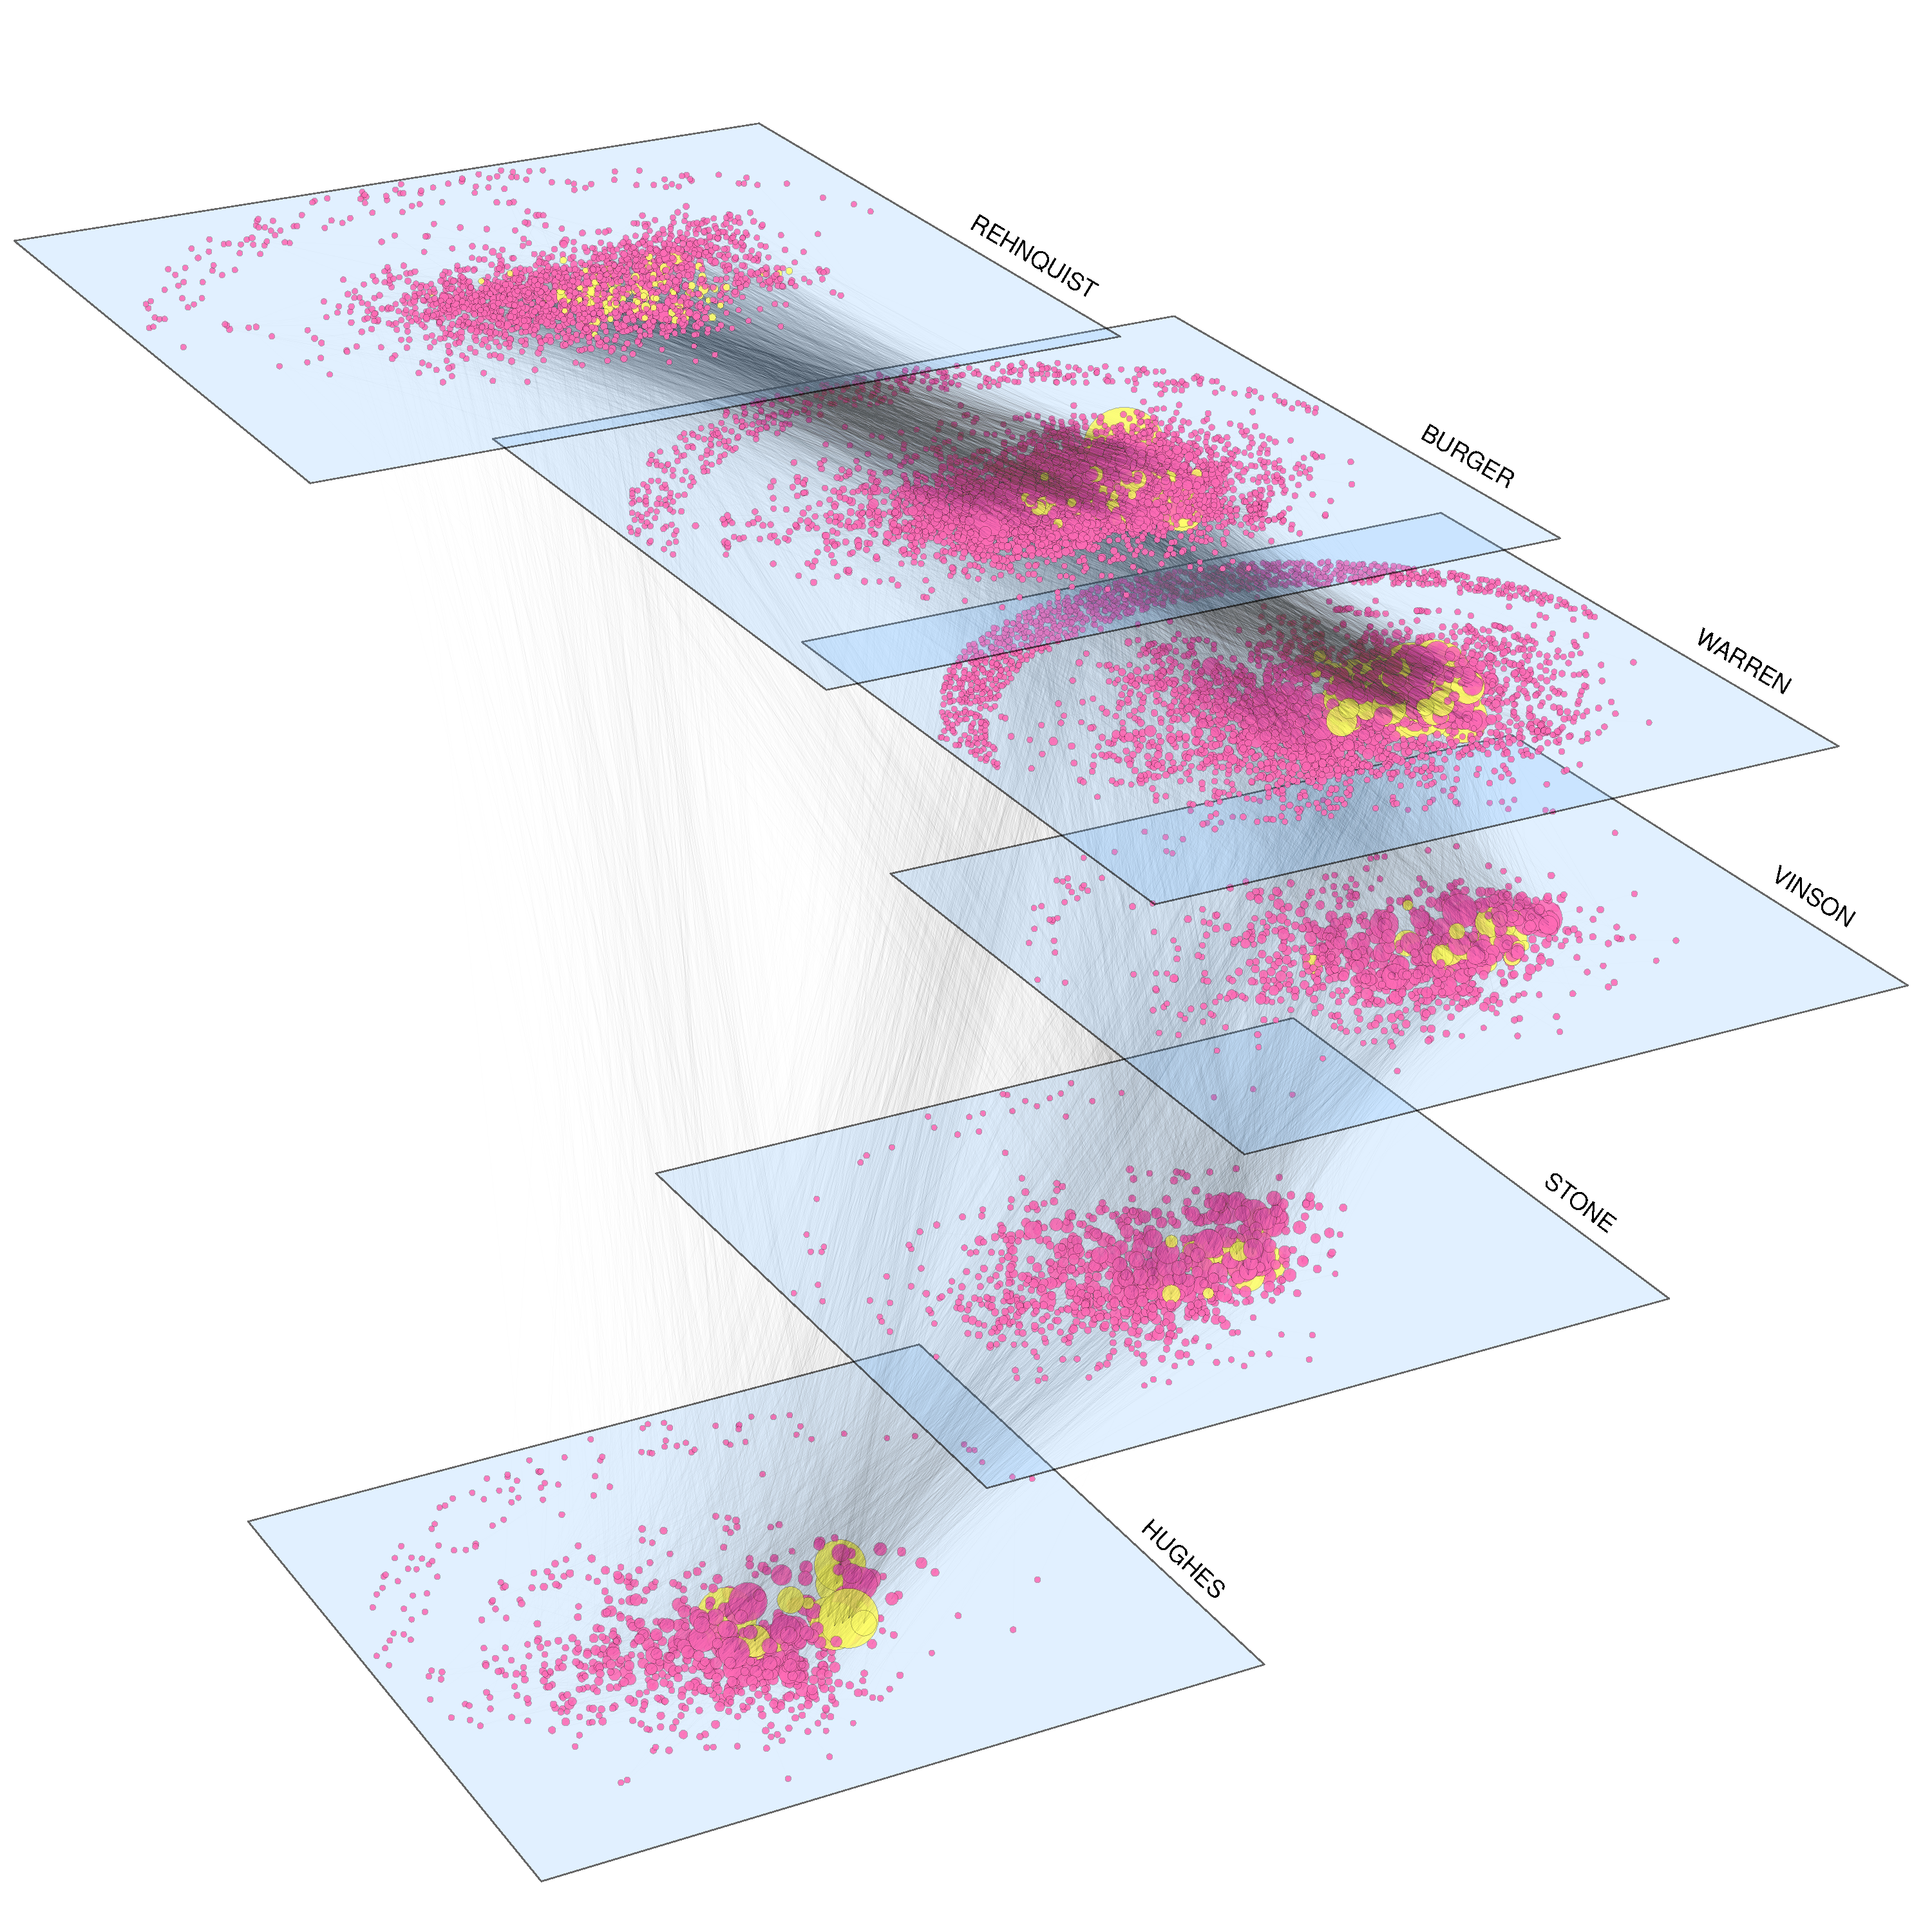
\includegraphics[scale=0.15,clip=true,trim=.5cm 0cm 0cm 2cm]{../../../NetworkVisualizations/citations1}
\end{column}

\end{columns}


\end{frame}

\begin{frame} \frametitle{Model Specification}

\begin{columns}
\begin{column}{5cm}
{\bf Exogenous Effects}
\begin{itemize}
\item Ideological Distance
\item Ideological Breadth
\item Same issue
\item Majority size
\item Issue area dummies
\end{itemize}
\end{column}

\begin{column}{6cm}
{\bf Dependence Effects}

\begin{itemize}
\item \# Mutual Dyads
\item \# Transitive Ties
\item \# In-two-stars
\item  \# Out-two-stars
\end{itemize}

\end{column}

\end{columns}


\end{frame}

\begin{frame} \frametitle{Results: Dependence}
\begin{changemargin}{-1cm}{-1cm}
\centering
 \begin{tabular}{cc}

    Reciprocity &  Transitivity \\
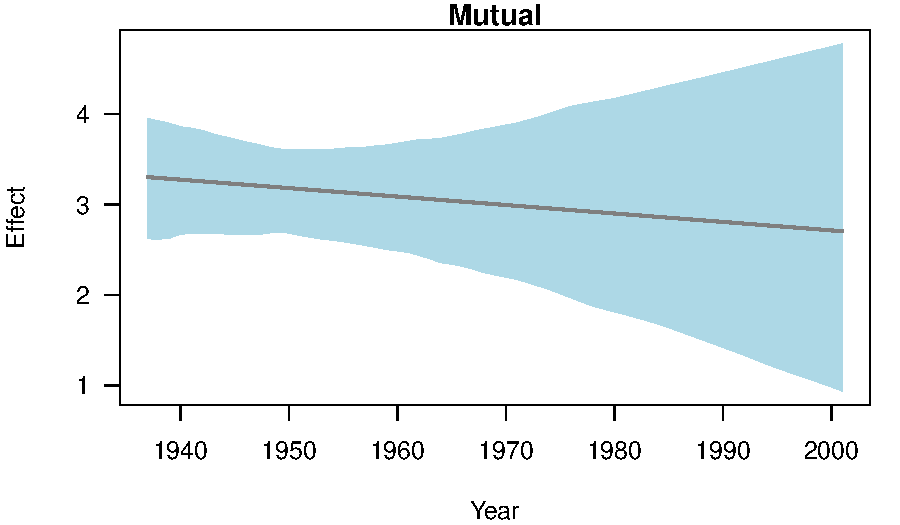
\includegraphics[width = 0.55\textwidth, trim= 1cm 1cm 0.5cm .45cm,clip=true]{../../images/mutual_coef_trend.pdf} & 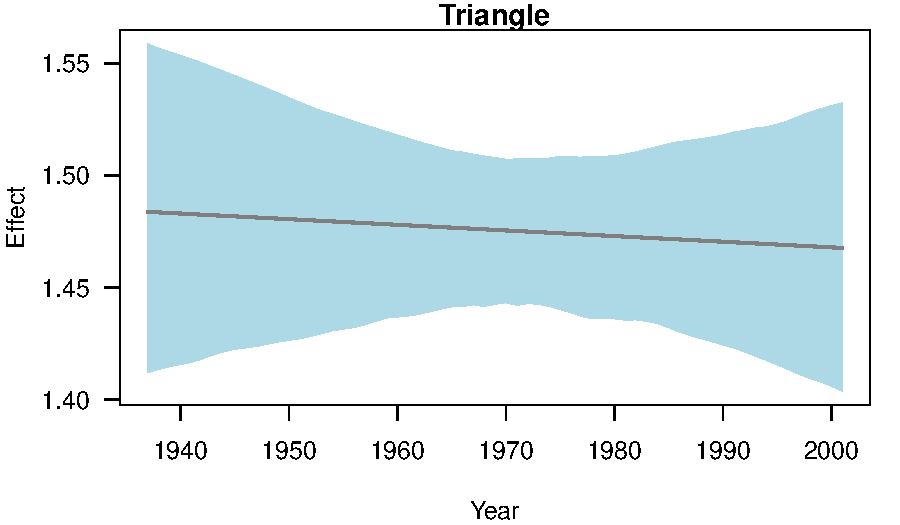
\includegraphics[width = 0.55\textwidth, trim= 1cm 1cm 0.5cm .45cm,clip=true]{../../images/triangle_coef_trend.pdf} \\
 
     Activity & Popularity \\
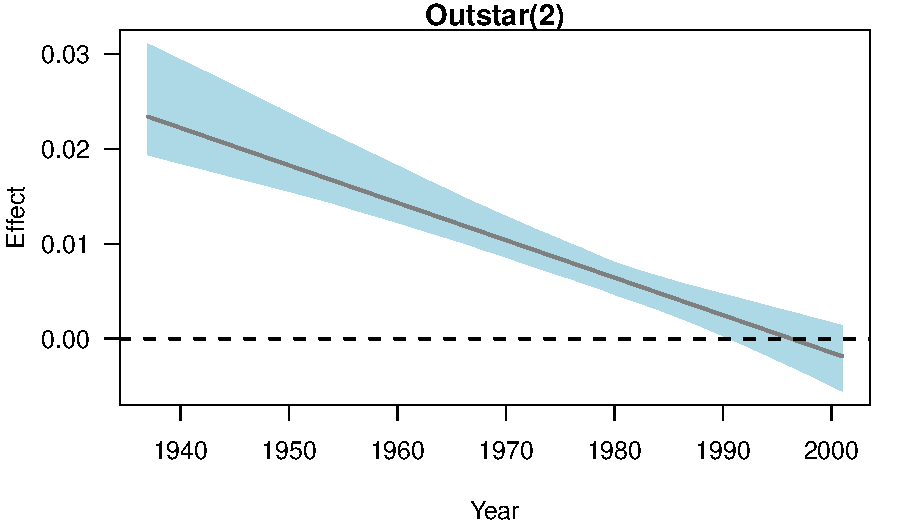
\includegraphics[width = 0.55\textwidth, trim= 1cm 1cm 0.5cm .45cm,clip=true]{../../images/o2star_coef_trend.pdf} & 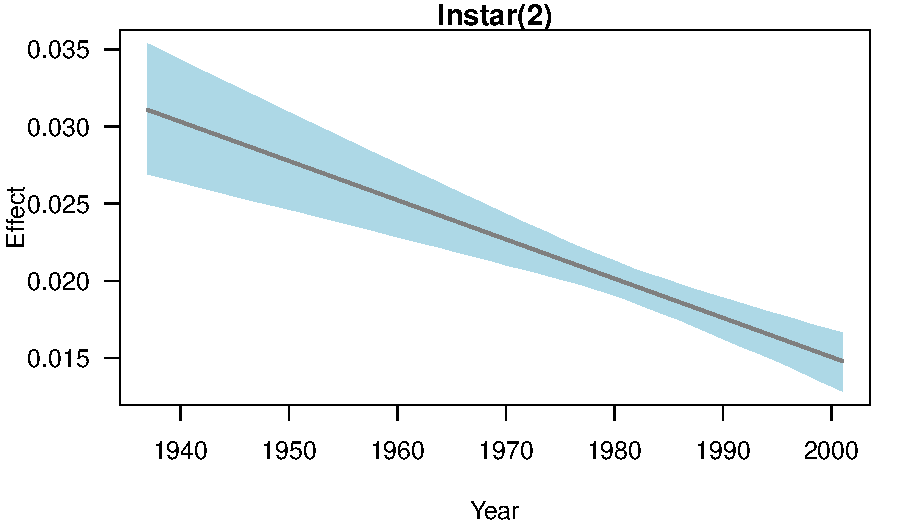
\includegraphics[width = 0.55\textwidth, trim= 1cm 1cm 0.5cm .45cm,clip=true]{../../images/i2star_coef_trend.pdf} \\
 
 
\end{tabular}

\end{changemargin}
\end{frame}

\begin{frame} \frametitle{Results: Covariates}
\begin{changemargin}{-1cm}{-1cm}
\centering

 \begin{tabular}{cc}
  MQ Score Difference & Ideological Breadth \\
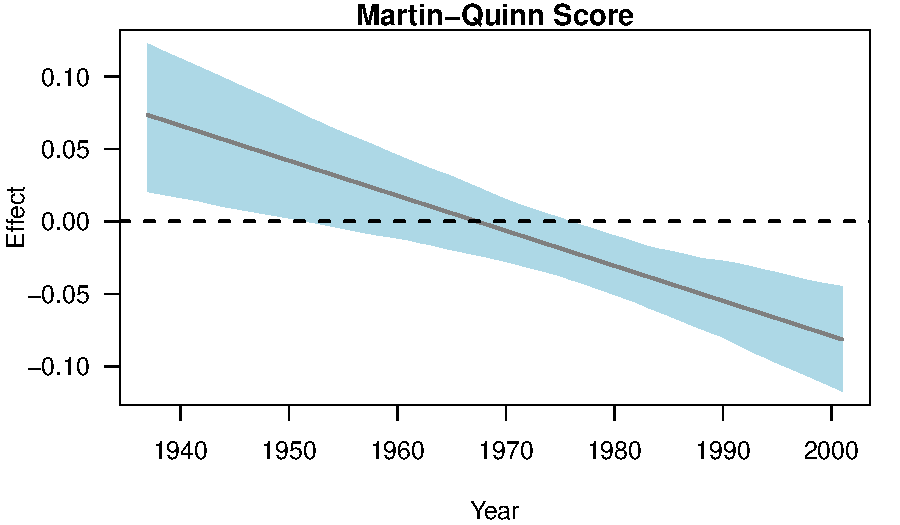
\includegraphics[width = 0.55\textwidth, trim= 1cm 1cm 0.5cm .45cm,clip=true]{../../images/mq_coef_trend.pdf} & 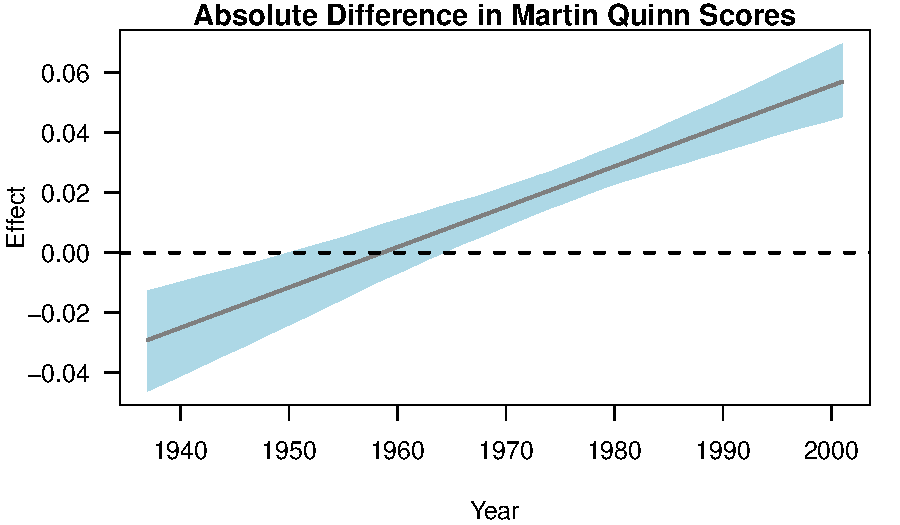
\includegraphics[width = 0.55\textwidth, trim= 1cm 1cm 0.5cm .45cm,clip=true]{../../images/absdiffmq_coef_trend.pdf} \\
 
   Same Issue &  Majority Size \\
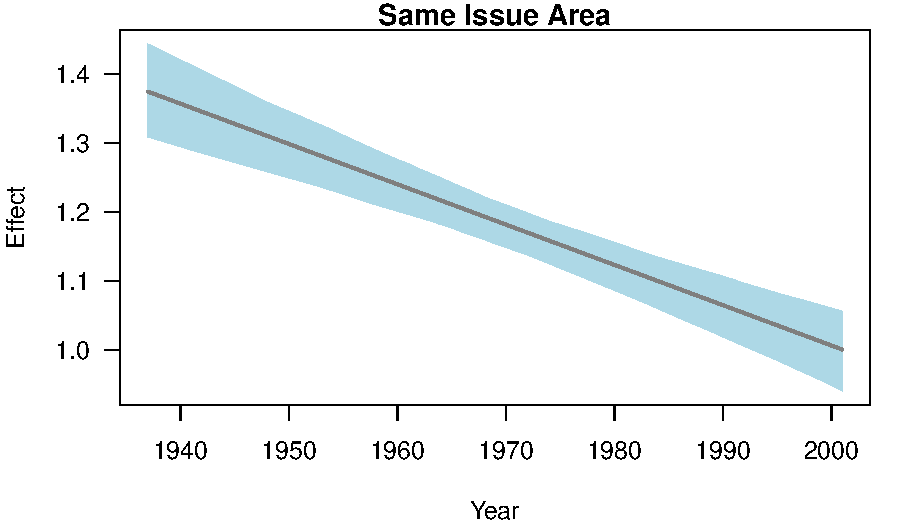
\includegraphics[width = 0.55\textwidth, trim= 1cm 1cm 0.5cm .45cm,clip=true]{../../images/sameissue_coef_trend.pdf} & 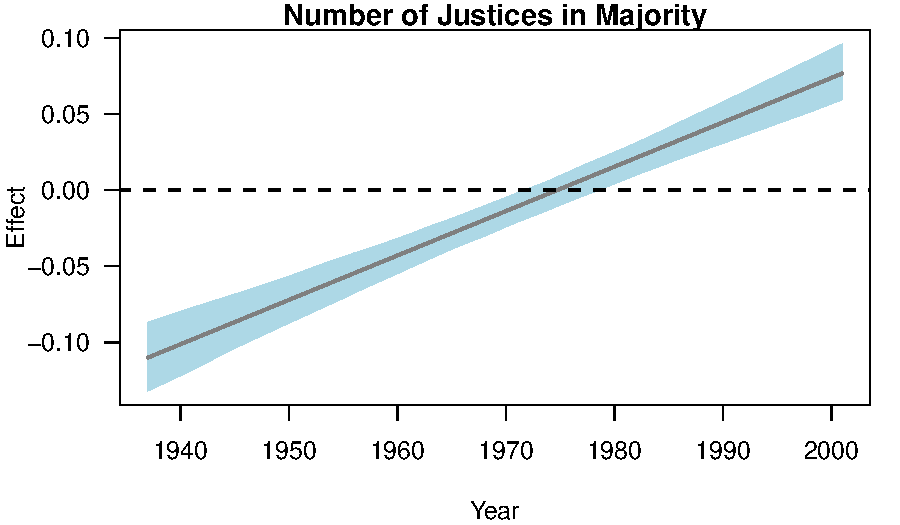
\includegraphics[width = 0.55\textwidth, trim= 1cm 1cm 0.5cm .45cm,clip=true]{../../images/numberjusticespro_coef_trend.pdf} \\
 
 
\end{tabular}

\end{changemargin}
\end{frame}

\begin{frame} \frametitle{Predictive Performance}

\begin{tabular}{rllll}
\hline \hline
& \multicolumn{2}{c}{Independent Model} & \multicolumn{2}{c}{Full Model} \\
  \hline
 & mean & range & mean & range \\ 
  \hline
precision & 0.5499 & (0.5384, 0.5619) & 0.8605 & (0.8526, 0.8666) \\ 
  recall & 0.0827 & (0.0811, 0.0843) & 0.5858 & (0.5817, 0.5891) \\ 
  F1 score & 0.1438 & (0.141, 0.1463) & 0.6971 & (0.6941, 0.7008) \\ 
   \hline \hline
\end{tabular}

\end{frame}

\begin{frame} \frametitle{Conclusion}

{\bf Key Findings}
\begin{enumerate}
\item Citation is characterized by reciprocity and transitivity
\item Dependence effects improve models of citations
\item c-TERGM represents comprehensive method
\end{enumerate}
~\\
{\bf Limitations}
\begin{enumerate}
\item Do not consider the signs of the citations
\item We miss recent terms
\item Case emergence considered exogenous
\end{enumerate}


\end{frame}

\end{document}









